% Chapter 6

\chapter{Issues in radiative correction calculation} % Chapter title

\label{ch:Issues} % For referencing the chapter elsewhere, use \autoref{ch:name}

%----------------------------------------------------------------------------------------

\section{Radiative Corrections related issues}

In the past, COMPASS has been using two programs for radiative corrections estimation: one is TERAD, a program that does analytic calculations of the ($x$,$y$)-dependent radiative correction factors, the other is RADGEN, which in addition to the ($x$,$y$)-dependent radiative correction factors allows one to take into account a kinematic smearing caused by the radiated photon. Despite being based on different QED calculation schemes, the two programs give compatible results for inclusive corrections.

Before going further in this discussion, some RADGEN formalism must be explained \cite{RADGEN}. The relations of the observed cross-section $\sigma_{meas}$ with the $1$-photon exchange cross-section $\sigma_{1\gamma}$ are, for the inclusive case:

\begin{equation}
    \sigma_{meas} = \delta_R(\Delta) (1+\delta_{vert}+\delta_{vac}+\delta_{sm})\sigma_{1\gamma}+\sigma_{el}+\sigma_{qel}+\sigma_{in}(\Delta),
\end{equation}

and for the semi-inclusive case:

\begin{equation}
    \sigma_{meas} = \delta_R(\Delta) (1+\delta_{vert}+\delta_{vac}+\delta_{sm})\sigma_{1\gamma}+\sigma_{in}(\Delta),
\end{equation}

where $\sigma_{1\gamma}$ is the one photon exchange Born cross-section and $\delta_{vac}$, $\delta_{vert}$ and $\delta_{sm}$ are corrections due to vacuum polarization by electron and muon pairs, vertex corrections and residuum of the cancellation of infrared divergent terms independent of the cut-off parameter $\Delta$:

\begin{equation}
  \begin{split}
    \delta_{vac} = \frac{\alpha}{\pi}\left[-\frac{20}{9}+\frac{2}{3}ln \frac{Q^2}{m_e^2}+\frac{2}{3}ln \frac{Q^2}{m^2_{\mu}}\right], \quad
    \delta_{vert} = \frac{\alpha}{\pi}\left[-2+\frac{3}{2}ln \frac{Q^2}{m^2}\right], \\
    \delta_{sm} = \frac{\alpha}{\pi}\left[-\frac{\pi^2}{6}+Li_2\left(cos^2 \frac{\theta}{2}\right)- \frac{1}{2}ln^2(1-y)\right],
  \end{split}
\end{equation}

where $m$ is the lepton mass and Li$_2$($x$) = $-\int_0^x ln(1-y)/y dy$ is the dilogarithm. The cross-sections $\sigma_{el}$, $\sigma_q$ and $\sigma_{in}$ are the contribution from radiative processes for elastic, quasielastic and deep inelastic scattering in case of nuclear targets. They can be calculated in terms of the radiative tail from $j^{th}$ mass level $\sigma_j$:
%
\begin{equation}
  \begin{split}
    \sigma_{el} = \sigma_{el}(M_A,1), \quad
    \sigma_{q} = \sigma_{q}(M,1), \quad
    \sigma_{in} = \int_{M+m_{\pi}}^W \frac{d\sigma_{in}(M_h,\theta_{max})}{dM_h},
  \end{split}
\end{equation}
%
where $M_h=\sqrt{W^2_{had}}$ and $\sigma_j$ ($j=el,\,q,\,in$) has the form of an integral over $\theta_{\gamma}$, the angle between the real and the virtual photons:
%
\begin{equation}
  \sigma_j(M,\theta_{max}) = \int_0^{\theta_{max}} T_0(W^j_2(T_1+T_2+T_3+T_4+T_5)+W^j_1(T_6+T_7))d\theta_{\gamma}.
\end{equation}
%
The structure functions $W^j_{1,2}$ have a different expressions for the different types of the tail. The termes $T_i$ are kinematical factors \cite{MoTsai}. $\theta_{max}$ is given as $\theta_{max} = min(\pi,\theta_{\Delta})$ where $\theta_{\Delta}$ is obtained via the relation:
%
\begin{equation}
  W^2_{had} = W^2 - 2\Delta(\nu+M-\sqrt{\nu^2+Q^2}cos(\theta_{\Delta})).
\end{equation}
%
The cut-off parameter $\Delta$ is introduced to divide the integration region over the photon energy in the soft and hard energy region. We already saw that the hard energy region $\sigma_{in}(\Delta)$ can be computed without any approximations. The correction factor for the soft energy part is given by:
%
\begin{equation}
  \delta_R(\Delta) = exp \left[-\frac{\alpha}{\pi}\left(ln \frac{E}{\Delta}+ln \frac{E'}{\Delta}\right)\left(ln \frac{Q^2}{m^2}-1\right)\right].
\end{equation}
%
In RADGEN the difference between the inclusive and semi-inclusive cross-section is only the elastic $\sigma_{el}$ and quasielactic $\sigma_{qel}$ cross-sections. The core of the problem is however in the calculation of $\sigma_{in}$. The semi-inclusive radiative corrections are given for the events with a hadron observed in the final state. The quantity $\sigma_{in}(M_{h},\theta_{max})$ is known and is not a problem but the lower limit of the integral is. In fact:
%
\begin{equation}
    W \geqslant M + M_{\pi},\quad E_{\gamma} \geqslant \frac{Q^2_{had}}{2M}+M_{\pi} \xrightarrow{Q^2_{had} \rightarrow 0} M_{\pi}
\end{equation}
%
As there must be energy conservation, photons with $\nu_{had} < 11$ GeV interacting with a proton at rest cannot produce a hadron with $12$ to $40$ GeV. This is the reason why we cannot use up to now TERAD for semi-inclusive correction calculation as it yields too large corrections. The same reasoning holds with RADGEN when it is not used as a generator. But used as a generator, it should be working and thus obviously there is a problem somewhere in the code of the generator.
%
\begin{figure}[htb]
\centerline{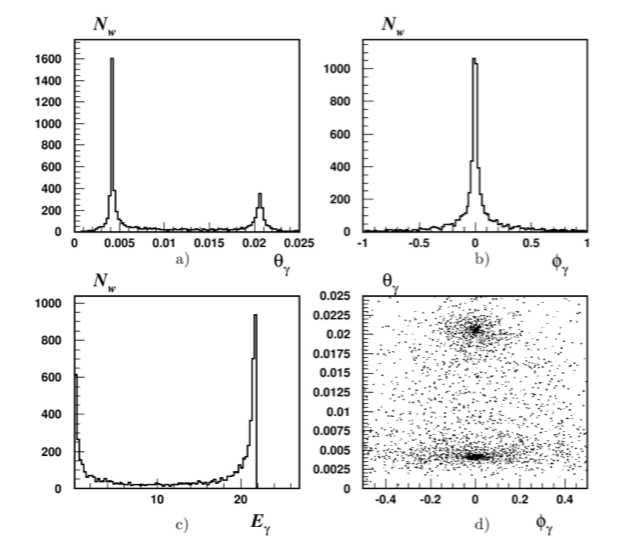
\epsfig{file=gfx/radgen.png,width=12cm}}
\caption{Distribution calculated by RADGEN for one point in HERMES kinematics ($x=0.1$, $y=0.8$, $E\approx27.5$ GeV, $\nu_{obs}\approx22$ GeV). The distribution of the radiation angles $\theta_{\gamma}$ a), $\phi_{\gamma}$ b) and of the energy c) of the radiated photon for $x=0.1$ and $y=0.8$. The two-dimensional distribution d) shows $\theta_{\gamma}$ vs $\phi_{\gamma}$. In panel c), one can note that the hard photon emissions are sizeable. Figure taken from \cite{RADGEN}}\label{fig:RAD}
\end{figure}

\begin{figure}[htb!]
\centerline{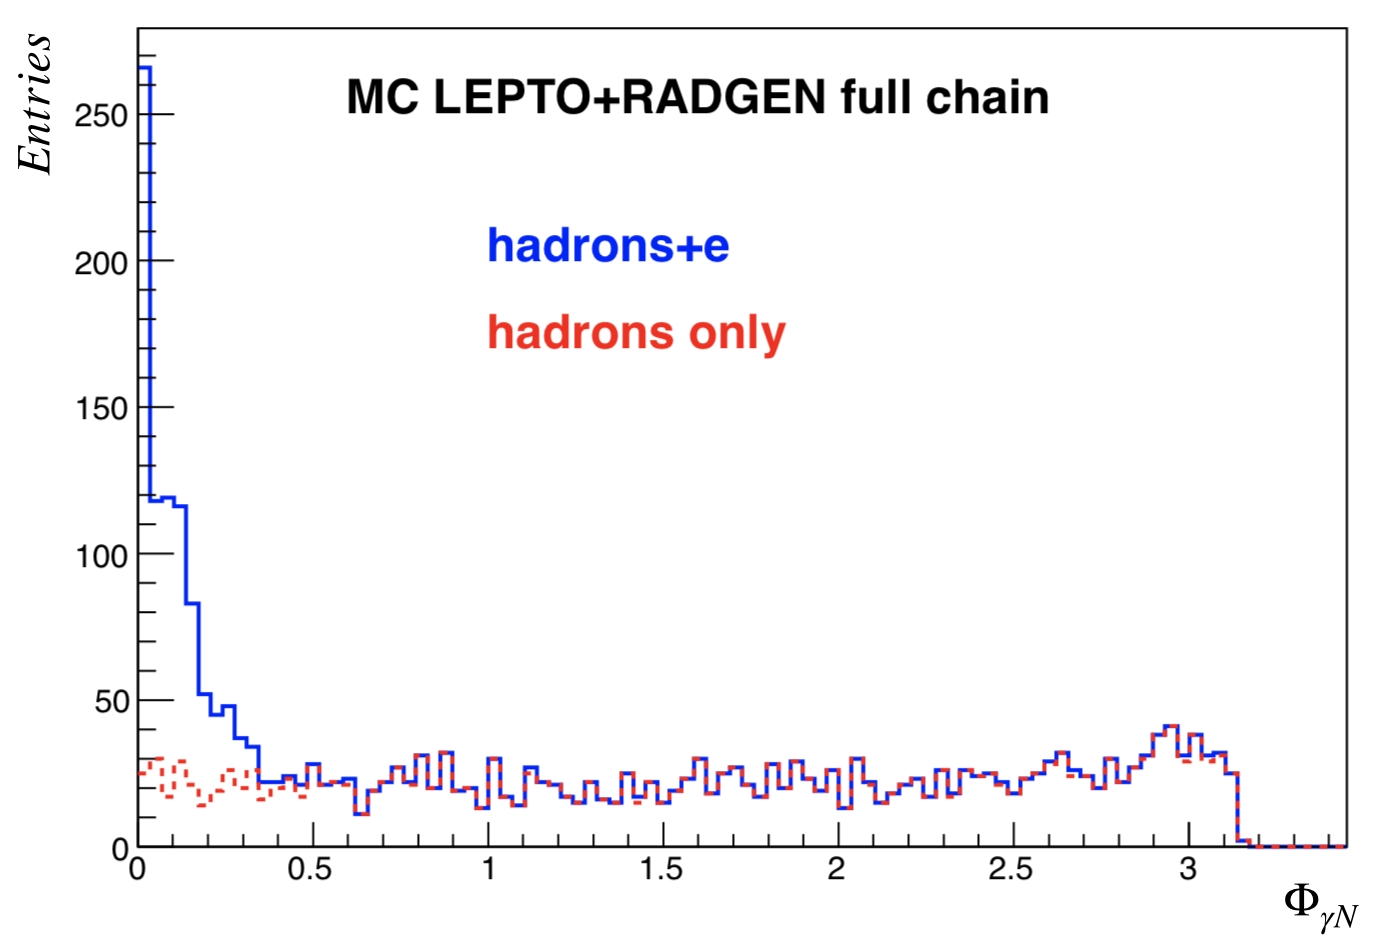
\epsfig{file=gfx/elprod.png,width=13.5cm}}
\caption{Hadron (red) and hadron+electron (blue) Monte-Carlo distributions versus $\Phi_{\gamma N}$ in the $\gamma$-nucleon reference plane. Figure taken from \cite{MarcinTalk}.}\label{fig:elprod}
\end{figure}

\begin{figure}[htb!]
\centerline{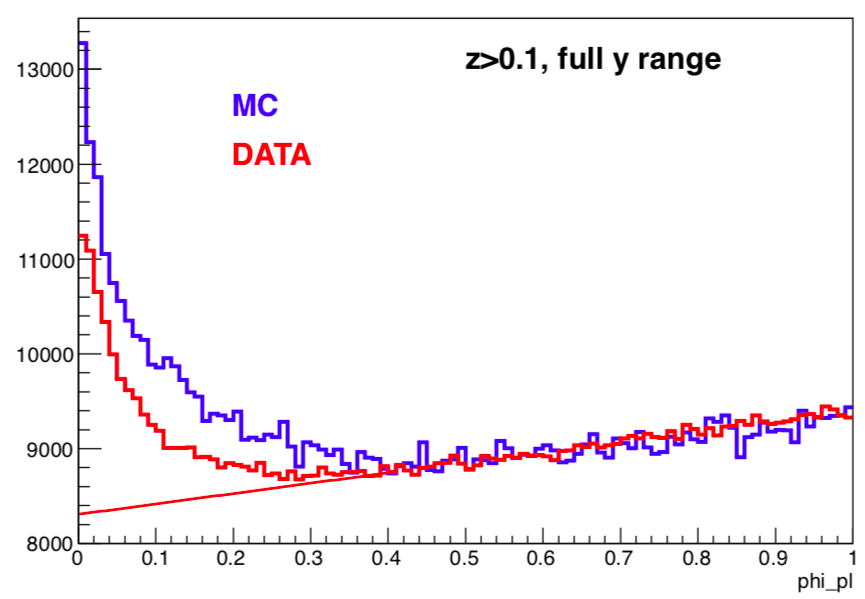
\epsfig{file=gfx/ph_pl.png,width=13.5cm}}
\caption{Electron distribution versus $\Phi_{\gamma N}$ in the $\gamma$-nucleon reference plane for 3 $< p_e <$ 8 GeV (region where RICH can discriminate electron in real data). Real Data are in red, Monte-Carlo with RADGEN in blue. Figure taken from \cite{MarcinTalk}.}\label{fig:ph_pl}
\end{figure}

When looking at the radiated photon energy distribution calculated by RADGEN for one point in HERMES kinematics ($x=0.1$, $y=0.8$, $E\approx27.5$ GeV, $\nu_{obs}\approx22$ GeV) as represented in the lower-left panel of Fig.~\ref{fig:RAD}, hard photon emissions are sizeable. The consequences of  having such radiated photon energy distribution can be investigated by looking at actual COMPASS data, e.g. $2006$ data. As the $^{6}$LiD target has a non-negligible radiation length part of photons will create $e^+e^-$ pairs and electrons from the conversion should be seen in the spectrometer. When performing Monte-Carlo generation with COMGEANT+RADGEN, a large amount of electrons is produced. Fig.~\ref{fig:elprod} shows the distribution of electrons and hadrons as a function of $\Phi_{\gamma N}$. The electrons are concentrated around $\Phi_{\gamma N} \sim 0$. By comparing the Monte-Carlo generation with the real data for electrons with $z>0.1$ and full $y$ range (Fig.~\ref{fig:ph_pl}), one can note that on average about $1.8$ more electrons are produced in Monte-Carlo than in real data.

%----------------------------------------------------------------------------------------

\section{Comparison between RADGEN and DJANGOH}

As one saw in the previous section, a rather problematic result is happening with RADGEN. The generator is producing a high number of hard photons leading to great discrepancies with the real data for the electron distribution. It is expected that DJANGOH will yield a better description of the data. As a first step the results of RADGEN and DJANGOH for the distribution of radiative photons are compared. In Fig.~\ref{fig:DJRAD}, the real photon energy $E_{\gamma}$ distributions are displayed for both generators for $0.8 \leq y \leq 0.9$ and $1 \leq Q^2 \leq 2 (GeV/c)^2$. One can see that overall, without comparing any number, DJANGOH is producing less hard photons than soft photons in contrast to RADGEN.

\begin{figure}[htb]
\centerline{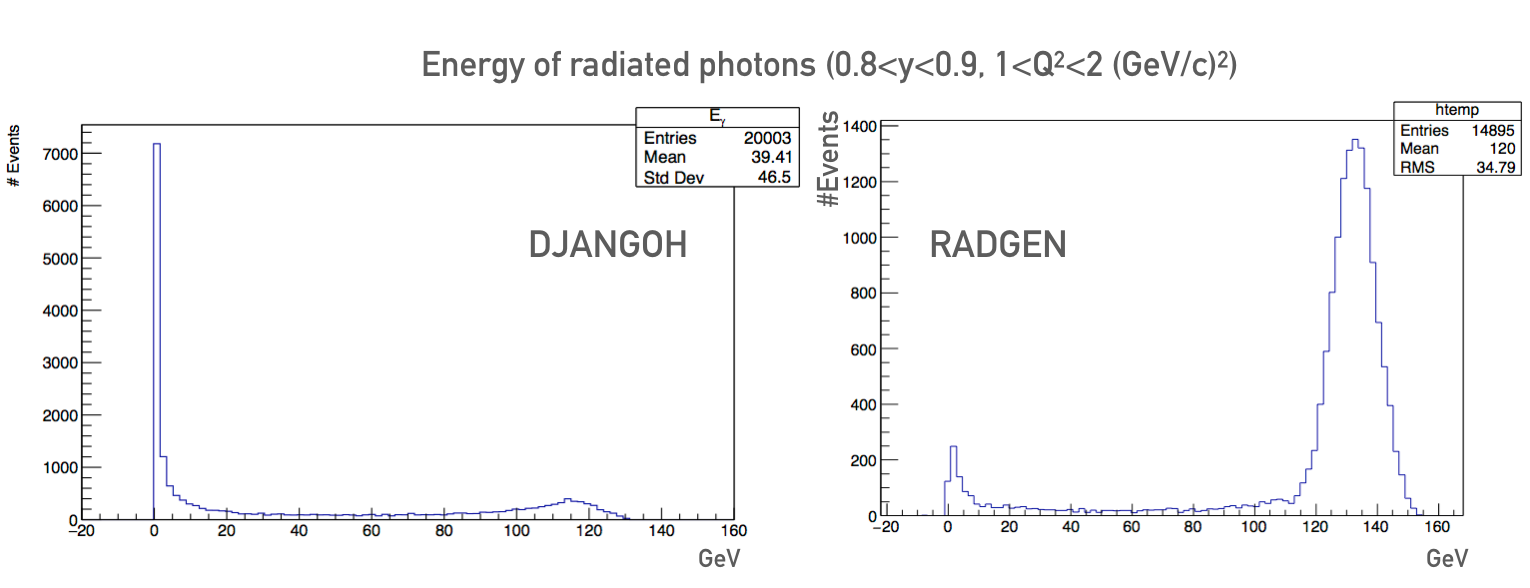
\epsfig{file=gfx/DJRAD.png,width=14.5cm}}
\caption{Left is the radiative photon energy distribution for $0.8 \leq y \leq 0.9$ and $1 \leq Q^2 \leq 2 (GeV/c)^2$ for DJANGOH, right is the same distribution for RADGEN. DJANGOH is producing overall more soft photons than hard ones, unlike RADGEN. Nevertheless, the plot does not allow to conclude whether DJANGOH is producing less hard photons than RADGEN.}\label{fig:DJRAD}
\end{figure}

By comparing more thoroughly, computing the proportion of radiative events in the range between 20 and 160 GeV over the total number of DIS events (Fig.~\ref{fig:tabDJRAD}), RADGEN has a total of $18.6$\% of event in this range when DJANGOH reaches a total of only $8.6$\%. We can then definitely claim that DJANGOH is producing less hard photons than RADGEN, which is encouraging for the comparison to real data.

\begin{figure}[htb]
\centerline{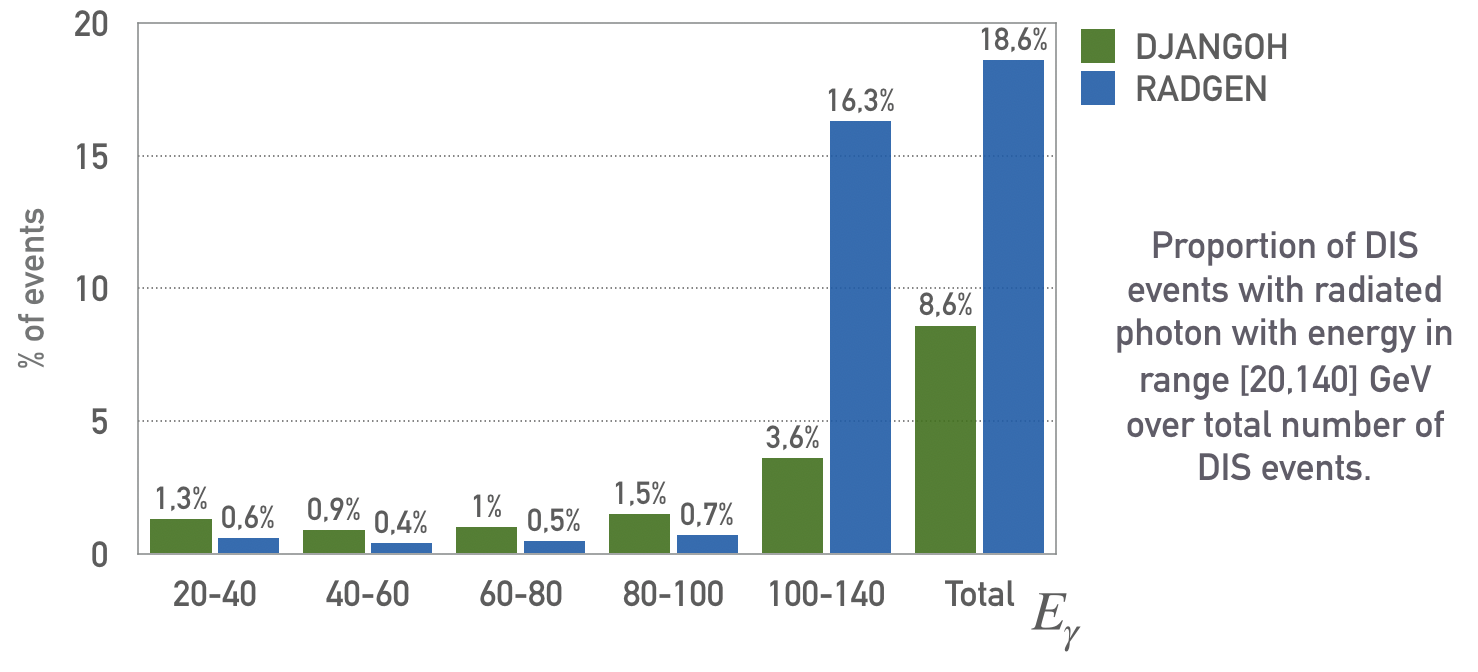
\epsfig{file=gfx/tabDJRAD.png,width=14cm}}
\caption{Comparison of proportion of event in high energy radiative photon range over total number of DIS event with the same kinematical restrictions as in Fig.~\ref{fig:DJRAD}. This comparison allows to conclude that DJANGOH is indeed producing less hard photons than RADGEN with more than a factor $2$ between the two generators. Thus, RADGEN is producing much less soft photons than DJANGOH, when referring to Fig.~\ref{fig:DJRAD}. Figure taken from \cite{DJANGOHnote}}\label{fig:tabDJRAD}
\end{figure}

\newpage

%----------------------------------------------------------------------------------------

\section{Summary}

RADGEN, when coupled to our MC simulation, was found not to be reproducing COMPASS data on the electron distribution. In fact it is producing a factor $1.8$ more electron than what is seen in real data. This is due to the fact that RADGEN produces more hard photons than soft photon, thus leading to a high electron production due to photon conversion in the target. A comparison was done between RADGEN and DJANGOH. It shows that DJANGOH is producing more soft photons than hard photons, but that it also produces less hard photons than RADGEN, leading to a smaller electron production. This gave us incentive to implement DJANGOH in our MC simulation and compare the results of MC to real data.
